\documentclass[11pt,a4paper]{article}
\usepackage[top=2cm,bottom=2cm,left=2.1cm,right=2.1cm]{geometry}
\usepackage[T1]{fontenc}
\usepackage{newtxtext,newtxmath}
\usepackage{microtype,amsmath,booktabs,array,tabularx,graphicx,xcolor,float,caption,enumitem,longtable}
\usepackage[colorlinks=true,linkcolor=blue!50!black,urlcolor=blue!50!black]{hyperref}
\usepackage{titlesec,fancyhdr}
\definecolor{navy}{HTML}{0B3D6B}
\titleformat{\section}{\Large\bfseries\color{navy}}{\thesection}{0.6em}{}
\titleformat{\subsection}{\large\bfseries\color{navy}}{\thesubsection}{0.6em}{}
\setlength{\parindent}{0pt}\setlength{\parskip}{5pt}
\newcolumntype{Y}{>{\raggedright\arraybackslash}X}
\pagestyle{fancy}\fancyhf{}\cfoot{\footnotesize LeakLens: dashboard and scenario guide \,|\, \thepage}\renewcommand{\headrulewidth}{0pt}
\captionsetup{font=small,labelfont=bf}
\newcommand{\term}[1]{\textbf{#1}}
\begin{document}
\begin{center}
{\Huge\bfseries\color{navy} LeakLens}\\[4pt]
{\Large Water Leak Localization System}\\[10pt]
{\LARGE Reading the Dashboard and How the Scenarios Work}\\[6pt]
{\normalsize Report 1 of 2 \,|\, B.Tech Project, IIIT Kottayam}
\end{center}
\vspace{2mm}\hrule\vspace{4mm}

\section{What this report is for}
This report explains, in plain language, (i) every word and element you see on the LeakLens dashboard, (ii) what each kind of scenario really does to a water network, (iii) the formulas behind each decision, and (iv) exactly how the ``Top-1'' result is calculated and compared across scenarios. Every number is taken from the project's own result files and is measured on \emph{held-out test scenarios} that the system never saw while learning (Section~\ref{sec:split}); all results are from simulation, not from real sensors.

\section{The dashboard, piece by piece}
\begin{figure}[H]\centering
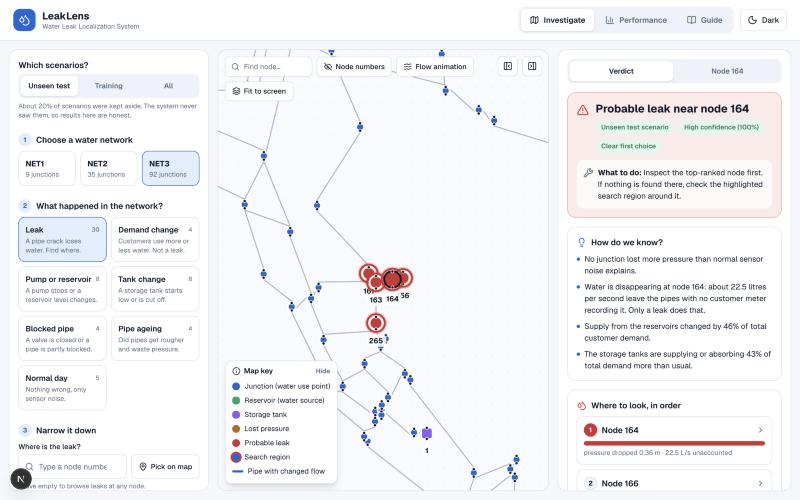
\includegraphics[width=\linewidth]{figures/ui_light_leak.jpg}
\caption{The Investigate screen after analysing a leak at node 115 (light theme). Left: choose a situation. Centre: network map. Right: verdict and reasons.}
\end{figure}

\subsection{Header}
\begin{itemize}[leftmargin=*,itemsep=2pt]
\item \term{LeakLens / Water Leak Localization System}: the project name and full title.
\item \term{Investigate}: pick a scenario and look at its result on the map. \term{Performance}: how well the system works over all scenarios. \term{Guide}: a short help page with the glossary.
\item \term{Light / Dark}: switches the colour theme. Your choice is remembered; the first time it follows your computer's setting.
\end{itemize}

\subsection{Left panel: three steps}
\begin{enumerate}[leftmargin=*,itemsep=2pt]
\item \term{Choose a water network.} NET1 (9 junctions, one pump, one tank), NET2 (35 junctions, one tank, no pumps), NET3 (92 junctions, 2 pumps, 3 tanks, 2 reservoirs). All three are standard EPANET benchmark networks.
\item \term{What happened in the network?} Seven kinds of situation: Leak, Demand change, Pump or reservoir, Tank change, Blocked pipe, Pipe ageing, Normal day. The small number on each card is how many scenarios of that kind exist for the chosen network.
\item \term{Narrow it down.} For leaks: \emph{Where is the leak?} (type a node number or press \emph{Pick on map}), \emph{How big?} (Tiny, Small, Medium, Large, Burst) and \emph{Conditions} (clean data, noisy sensors, hidden behind another event, starts at another time). The counter shows how many scenarios match; \emph{Surprise me} runs a random one. Other kinds are searched by words such as ``pump'' or ``30\%''.
\end{enumerate}
\term{Customers have smart demand meters} tells the system whether the water used at each node is known. \term{Analyse this scenario} runs the analysis.

\subsection{Map}
Each circle is a \term{junction} (a point where customers draw water), squares are \term{reservoirs} (green, sources) and \term{tanks} (purple, storage). Lines are pipes. After an analysis: red circles are the predicted leak nodes (largest = first choice); orange circles lost pressure; red rings mark the \term{search region}; blue pipes carried a different flow than on a normal day. Click any node to see its pressure over the day.

\subsection{Right panel: the verdict}
\begin{description}[leftmargin=*,itemsep=2pt]
\item[Verdict box] The cause found (for example ``Probable leak near node 115'') with a confidence label and a \emph{What to do} sentence.
\item[Confidence] High if the model gives its answer at least 85\% probability, Medium from 60\%, otherwise Low. It is a model score, not a guarantee.
\item[Clear first choice / Close call] ``Clear'' when the second-ranked node scores less than half of the first; otherwise the first nodes are close and several should be checked.
\item[How do we know?] Plain-English reasons, built from the measurements: how many junctions lost pressure, whether water disappears without a meter noticing, whether a pump lost flow, and so on.
\item[Where to look, in order] The five highest-scoring nodes. The bar shows each node's score relative to the first.
\item[Check against the answer key] Because the data are simulated we know the true cause and the true leak node, so the dashboard shows whether the cause was right and whether Top-1 was hit (or how many pipes away it missed).
\item[Technical details] The probability of every cause, the 14 numbers the model looked at, and the score formula.
\item[Node tab] Pressure and unaccounted flow at the selected node, and a chart of pressure over 24 hours on the normal day versus this scenario.
\end{description}

\subsection{Glossary of terms on screen}
\begin{center}\small
\begin{tabularx}{\linewidth}{@{}>{\bfseries}p{3.1cm}Y@{}}
\toprule
Term & Meaning \\
\midrule
Pressure (m) & How hard water pushes in the pipe, written as metres of water column. Leaks and heavy use lower it. \\
Flow (L/s) & Litres of water moving through a pipe each second. \\
Baseline / normal day & The simulated day with nothing wrong. Every scenario is compared with it. \\
Sensor noise & Small random errors in real readings. The system learns their size so it does not raise alarms for them. \\
Unaccounted flow & Water leaving a node that no customer meter records. This is the leak flow. \\
Demand meters & Meters that report how much water customers draw at each node. \\
Leak score & Number used to rank nodes: unaccounted flow plus pressure drop, each scaled to 0--1. \\
Top-1 / Top-5 & The real leak is the first node on the list / among the first five. \\
Pipe hops & Number of pipes between the predicted node and the real leak (0 = exact). \\
Search region & The predicted node and the nodes directly connected to it. \\
Confidence & How strongly the classifier prefers its answer over the other causes. \\
\bottomrule
\end{tabularx}
\end{center}

\section{What a scenario is}
A scenario is one 24-hour simulation of a network in which one thing (or a few things together) is changed from the normal day. The normal day is simulated first and called the \emph{baseline}. Each scenario is stored with its true answer (which kind of event and, for leaks, which node), used only to score the system. The project contains 617 scenarios, split about 80\% for learning and 20\% for testing (Section~\ref{sec:split}).

\begin{center}\small
\begin{tabularx}{\linewidth}{@{}>{\bfseries}p{2.8cm}p{1.5cm}Y@{}}
\toprule
Kind & Count & What is changed \\
\midrule
Leak & 299 & A hole of area $A$ opens at one junction at a given hour. Sizes: Tiny 0.0001, Small 0.0003, Medium 0.001, Large 0.003, Burst 0.01 m$^2$. Variants: every junction, five sizes, four start times (2, 8, 12, 20 h), sensor noise, and hidden behind another event. \\
Demand change & 60 & Water use at one node $\times$1.5 or $\times$0.5; all nodes $\times$1.3 or $\times$0.7; a hydrant opened for four hours. \\
Pump / reservoir & 54 & A pump switched off for 2, 4 or 6 hours while it normally runs; a reservoir head raised or lowered by 2, 5 or 10 m. \\
Tank change & 60 & A tank starts at 10--90\% full, or is cut off from the network. \\
Blocked pipe & 48 & A busy pipe is closed at 10:00, or is partly blocked (large minor loss). \\
Pipe ageing & 42 & Every pipe becomes rougher (Hazen--Williams $C$ multiplied by 0.6 to 0.95). \\
Normal day & 54 & Nothing changes; only measurement noise (small or large) or none at all. \\
\bottomrule
\end{tabularx}
\end{center}
Most non-leak scenarios also exist in a ``noisy'' copy, so the model sees realistic readings.

\section{How each scenario changes the network}
All scenarios are simulated by the EPANET engine through WNTR with pressure-dependent demand. Three tables are recorded for each hour: pressure at every node, flow in every pipe and the demand actually delivered at every node (what a customer meter would read).

\subsection{Leak}
Water escapes through an orifice. With discharge coefficient $C_d=0.75$, leak area $A$, gravity $g$ and gauge pressure head $P$ at the node,
\begin{equation}\label{eq:leak}
Q_\ell(t)=C_d\,A\,\sqrt{2\,g\,P(t)}\qquad (t\ge t_{\text{start}}).
\end{equation}
The leak pulls extra water into that node, so flow rises in the pipes leading to it and pressure falls around it, most at the leak node. Because $Q_\ell$ grows with pressure, leaks at low-lying, high-pressure nodes lose more water. A leak is \emph{local} (largest effect at one node) and \emph{unmetered}.

\subsection{Demand change}
Customer use at node $i$ is $D_i(t)=D_{\text{base},i}\,m(t)\,f$, where $m(t)$ is the daily pattern and $f$ the scenario factor. More use pulls more flow through the pipes and lowers pressure nearby, like a leak, but the extra flow is \emph{metered}: customers are drawing it.

\subsection{Pump outage, reservoir head, tank level}
These change the network's \emph{boundary conditions}, the places where water and pressure enter. Switching a pump off removes the energy it adds, so pressure falls across everything it serves, tanks start to supply instead, and the pump's flow goes to zero. Raising or lowering a reservoir head by $\Delta h$ shifts the pressure of the whole connected network by about $\Delta h$. A tank that starts low supplies less pressure and exchanges flow with the pipes. None of these lose water, and each affects \emph{many} nodes at once.

\subsection{Blocked pipe}
Closing a pipe forces its flow elsewhere. Nodes downstream lose pressure, nodes upstream can gain it, and flows in neighbouring pipes change. No water is lost.

\subsection{Pipe ageing}
Older pipes are rougher. In the Hazen--Williams head-loss law
\begin{equation}
h_f=\frac{10.67\,L\,Q^{1.852}}{C^{1.852}\,d^{4.87}},
\end{equation}
a smaller roughness coefficient $C$ means more pressure lost for the same flow. Pressure falls slowly and widely, and most where flow is highest. No water is lost.

\subsection{What it looks like in the data}
\begin{figure}[H]\centering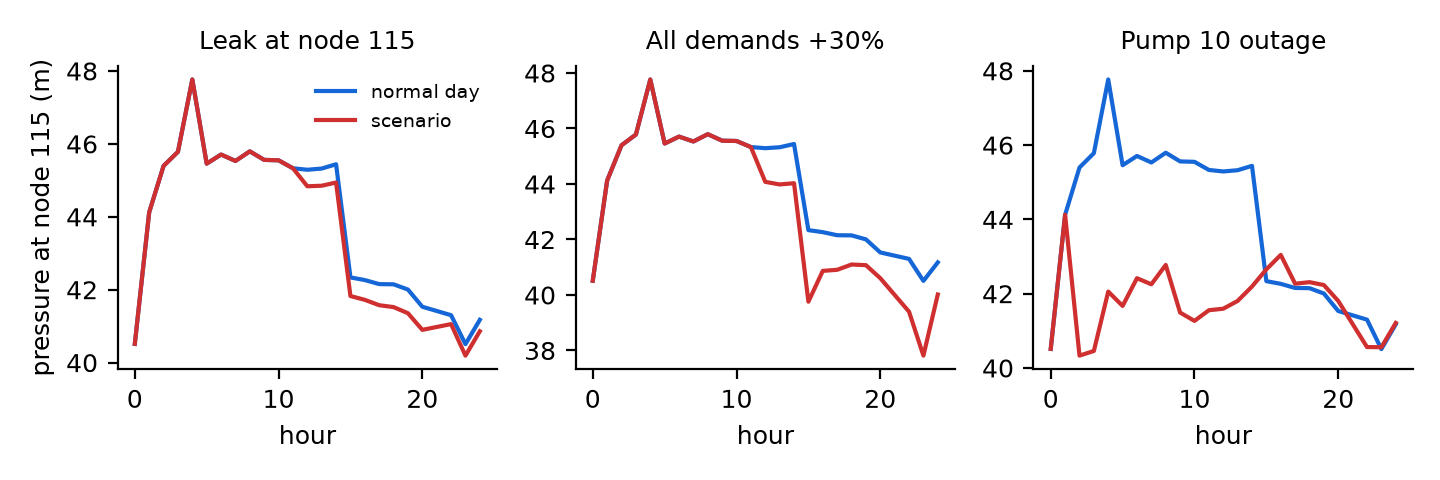
\includegraphics[width=\linewidth]{figures/fig_pressure.png}
\caption{Pressure at NET3 node 115 on a normal day (blue) and in three scenarios (red). The leak causes a step down from hour 12; the demand surge lowers pressure all day; the pump outage drops it sharply while the pump is off.}\end{figure}

Typical size of the effect, measured over all scenarios of each kind (median). \emph{Drop} is the worst pressure drop at any junction; \emph{Hit} is the share of junctions that lost more pressure than sensor noise explains; \emph{Unacc.} is the largest unaccounted flow in multiples of its noise level.
{\small\begin{longtable}{@{}llrrrr@{}}
\toprule
Network & Kind & Scenarios & Drop (m) & Hit & Unacc. \\
\midrule
\endhead
NET1 & Pipe ageing & 14 & 9.97 & 100\% & 0.1 \\
NET1 & Demand change & 20 & 1.00 & 72\% & 0.1 \\
NET1 & Leak & 57 & 3.04 & 100\% & 22.4 \\
NET1 & Normal & 18 & 0.09 & 0\% & 0.2 \\
NET1 & Pump / reservoir & 18 & 0.28 & 0\% & 0.1 \\
NET1 & Tank change & 12 & 9.91 & 100\% & 0.1 \\
NET1 & Blocked pipe & 16 & 4.30 & 33\% & 0.1 \\
NET2 & Pipe ageing & 14 & 0.29 & 0\% & 0.1 \\
NET2 & Demand change & 20 & 0.11 & 0\% & 0.1 \\
NET2 & Leak & 91 & 74.12 & 100\% & 14.6 \\
NET2 & Normal & 18 & 0.10 & 0\% & 0.2 \\
NET2 & Tank change & 12 & 0.57 & 50\% & 0.1 \\
NET2 & Blocked pipe & 16 & 0.17 & 0\% & 0.1 \\
NET3 & Pipe ageing & 14 & 5.84 & 98\% & 0.1 \\
NET3 & Demand change & 20 & 0.14 & 0\% & 0.1 \\
NET3 & Leak & 151 & 0.77 & 2\% & 7.9 \\
NET3 & Normal & 18 & 0.13 & 0\% & 0.3 \\
NET3 & Pump / reservoir & 36 & 1.92 & 1\% & 0.1 \\
NET3 & Tank change & 36 & 2.49 & 32\% & 0.1 \\
NET3 & Blocked pipe & 16 & 7.53 & 55\% & 0.1 \\
\bottomrule
\end{longtable}}
Two things stand out: only leaks show a large unaccounted flow, and non-leak events either spread over most junctions (pumps, tanks, ageing, blockage) or are matched by customer meters (demand).

\section{From measurements to a decision}
\subsection{Step 1: compare with the normal day}
For node $i$ and hour $t$ the \emph{pressure residual} is
\begin{equation}
r_i(t)=P^{\text{normal}}_i(t)-P^{\text{observed}}_i(t).
\end{equation}
A reading only counts if the residual stays above the threshold for two consecutive hours (\emph{persistence}), so one noisy reading cannot trigger anything. The peak persistent drop is $d_i=\max_t \min\{r_i(t),r_i(t{+}1)\}$.

\subsection{Step 2: learn the noise}
Each network has 18 normal runs containing only sensor noise; the learning (training) ones, about 14 per network, are used here. The pressure threshold is learned as
\begin{equation}
\tau_P=\max\{0.1,\;4\,\sigma_P\},
\end{equation}
where $\sigma_P$ is the standard deviation of those residuals ($\tau_P\approx 0.5$--$0.6$ m in all three networks). Flow and demand noise are learned in the same way. A fixed 0.5 m threshold, by contrast, raised an alarm on 41.7\% of the normal test days.

\subsection{Step 3: follow the water}
Water cannot appear or vanish at a junction. For junction $i$, with pipe flows $Q_p$ signed $+1$ if the pipe ends at $i$ and $-1$ if it starts there,
\begin{equation}
\sum_{p}\operatorname{sign}(p,i)\,Q_p(t)=D_i(t)+Q_{\ell,i}(t).
\end{equation}
Subtracting the normal day and the change in metered demand leaves the leak:
\begin{equation}\label{eq:unacc}
u_i(t)=\Big[\sum_p \operatorname{sign}(p,i)\,\Delta Q_p(t)\Big]-\Delta D_i(t)\;=\;Q_{\ell,i}(t).
\end{equation}
In noise-free data $u_i$ is exactly the leak flow at node $i$ and zero elsewhere. A demand change cancels in (\ref{eq:unacc}) because it is metered. Pressure and unaccounted flow are divided by their noise thresholds, so a value of 1 means ``at the noise limit''.
\begin{figure}[H]\centering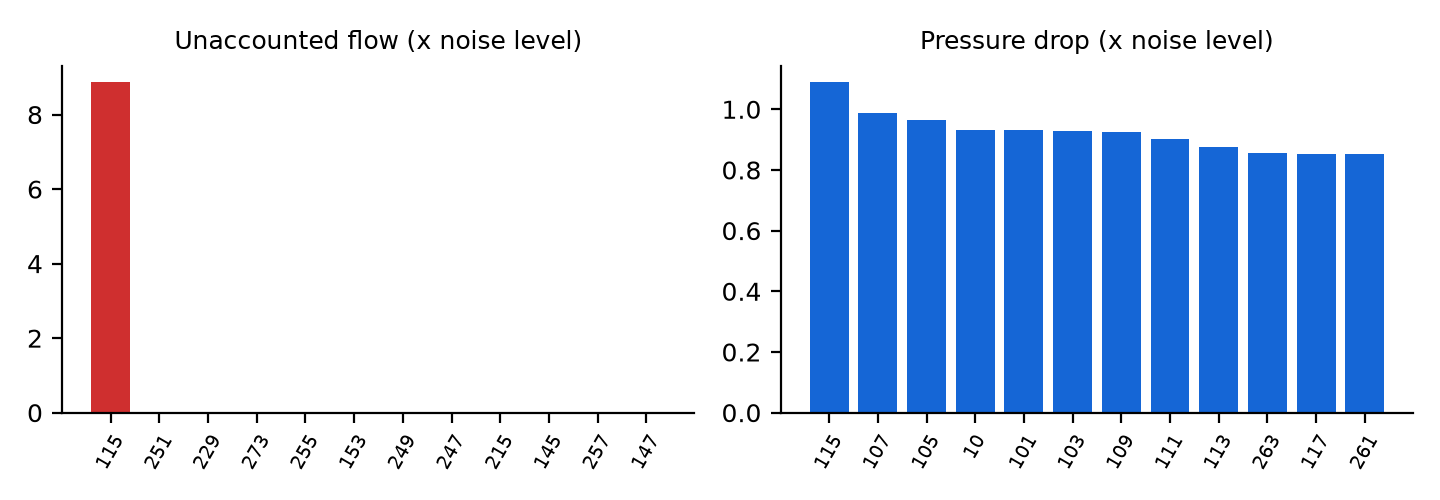
\includegraphics[width=\linewidth]{figures/fig_signals.png}
\caption{Leak at NET3 node 115. Left: unaccounted flow is large at node 115 and essentially zero elsewhere. Right: the pressure drop is high at 115 but also high at its neighbours, so pressure alone is a blurrier signal.}\end{figure}

\subsection{Step 4: fourteen summary numbers}
Each scenario is summarised by 14 numbers, for example the share of junctions with a pressure drop, the largest unaccounted flow, the pump flow lost, and the change in reservoir supply and tank flow. Median values by kind of event:
{\small\begin{center}\begin{tabular}{@{}p{5.6cm}rrrrrrr@{}}
\toprule
Number & Normal & Leak & Demand & Pump/res. & Tank & Blocked & Ageing \\
\midrule
Biggest pressure drop / noise threshold & 0.20 & 4.25 & 1.11 & 2.61 & 4.29 & 6.82 & 4.28 \\
Share of junctions with a pressure drop & 0.00 & 0.56 & 0.03 & 0.01 & 0.82 & 0.44 & 0.96 \\
Biggest unaccounted flow / noise & 0.25 & 11.16 & 0.06 & 0.08 & 0.05 & 0.07 & 0.06 \\
Share of nodes with changed metered demand & 0.00 & 0.00 & 0.03 & 0.00 & 0.00 & 0.00 & 0.00 \\
Pump flow lost (1 = off) & 0.01 & 0.00 & 0.00 & 0.09 & 0.75 & 0.01 & 0.16 \\
Reservoir supply change / total demand & 0.01 & 0.01 & 0.01 & 0.37 & 0.46 & 0.01 & 0.34 \\
Tank flow change / total demand & 0.01 & 0.43 & 0.23 & 0.37 & 0.46 & 0.01 & 0.34 \\
Biggest pressure rise / noise & 0.20 & 0.54 & 0.44 & 2.62 & 3.20 & 3.29 & 6.28 \\
Share of pipes with changed flow & 0.00 & 0.60 & 0.35 & 0.47 & 0.60 & 0.65 & 0.81 \\
\bottomrule
\end{tabular}\end{center}}

\subsection{Step 5: normal, or something else?}
If every signal is within noise (all ratios below 1, almost no pipe flow change, no metered demand change) the answer is \term{normal}. This is the quiet gate; it is why normal days raise no false alarms, and also why very small leaks are reported as normal.

\subsection{Step 6: which cause?}
A random forest of 300 decision trees votes on the 14 numbers and outputs a probability for each of the six causes. The highest is the verdict; its probability gives the confidence label. Accuracy is measured on the held-out test scenarios only.

\section{How the system is trained and tested}\label{sec:split}
If a system is tested on the same scenarios it learned from, it will look perfect and we learn nothing. So all 617 scenarios were split once, with a fixed random seed, into about \textbf{80\% for learning (478 scenarios)} and about \textbf{20\% for testing (139 scenarios)}.
\begin{itemize}[leftmargin=*,itemsep=2pt]
\item \textbf{Learned from the training scenarios only:} the noise thresholds (from the normal training runs) and the cause classifier (the random forest).
\item \textbf{Not learned at all:} the leak ranking of equation (\ref{eq:score}) is a fixed formula; its settings were chosen during development, before this split.
\item \textbf{Measured on the test scenarios only:} every accuracy, false-alarm and Top-$k$ figure in this report.
\item \textbf{Near-copies stay together.} All leaks at the same junction (every size, start time, noise level and ``hidden behind'' variant) go to the same side, and a scenario and its sensor-noise twin go to the same side. Otherwise the test would be too easy.
\item \textbf{Stratified.} Each network and each kind of event is split about 80/20; the test set has 12 scenarios of every non-leak kind and 67 leaks.
\item \textbf{Dashboard tags.} Every scenario shows \emph{Unseen test} or \emph{Training}. Only the unseen ones give an honest check; the picker shows them by default.
\end{itemize}
\textbf{Training versus test.} Cause accuracy is 95.6\% on the training scenarios and 82.7\% on the unseen test scenarios, the gap you expect when a model has partly memorised; leak Top-1 is 97.8\% on training leaks and 96.7\% on test leaks, nearly the same, because the ranking is not trained.

\section{How Top-1 is calculated}
\subsection{Scoring the nodes}
Only if the verdict is ``leak'' are nodes ranked. For each junction $i$ the two signals are scaled to 0--1 by dividing by their largest value in the network, $A_i=u_i^{\text{peak}}/\max_j u_j^{\text{peak}}$ and $D_i=d_i/\max_j d_j$, and combined:
\begin{equation}\label{eq:score}
S_i=A_i+0.3\,D_i .
\end{equation}
The unaccounted flow is the main signal; pressure drop is a backup that matters when flow data are noisy. If no node has an unaccounted flow above its noise limit, only the pressure term is used. Nodes are sorted by $S_i$ from highest to lowest.

\subsection{Worked example (NET3, leak at node 115)}
The pressure threshold is 0.58 m. Node 115 has both the largest unaccounted flow and the largest pressure drop, so $A=1.00$, $D=1.00$ and $S=1.00+0.3\cdot1.00=1.30$. Its neighbours have almost no unaccounted flow but a large pressure drop:
\begin{center}\begin{tabular}{@{}rcccc@{}}\toprule
Rank & Node & $A$ & $D$ & Score $S$ \\\midrule
1 & 115 & 1.00 & 1.00 & 1.30 \\
2 & 107 & 0.00 & 0.91 & 0.27 \\
3 & 105 & 0.00 & 0.89 & 0.27 \\
\bottomrule\end{tabular}\end{center}
The true node, 115, is ranked first, so this scenario counts as a Top-1 success: 0 pipe hops from the truth.

\subsection{Rank, Top-$k$ and error}
For leak scenario $s$ with true node $n_s$, let $r_s$ be the position of $n_s$ in the sorted list ($r_s=1$ means first). Then
\begin{equation}
\text{Top-}k=\frac{1}{N}\sum_{s=1}^{N}\mathbf{1}[\,r_s\le k\,],
\qquad
\text{error}_s=\text{hops}\big(\hat n_s,n_s\big),
\end{equation}
where $\hat n_s$ is the first-ranked node and hops is the number of pipes on the shortest path between the two nodes (the length in metres is also recorded). Over the 60 test leak scenarios scored, the true node was ranked first 58 times, so Top-1 $=58/60=$ 96.7\%. The first version of the system managed 35 of 60 (58.3\%). With only 60 test leaks, one miss moves the percentage by about 1.7 points, so read small differences loosely.

\subsection{Why Top-1 differs between scenarios}
\begin{center}\small\begin{tabular}{@{}lcccc@{}}\toprule
Method & Top-1 & Top-3 & Top-5 & Mean hops \\\midrule
First version & 58.3\% & 70.0\% & 71.7\% & 3.35 \\
Final method & 96.7\% & 98.3\% & 98.3\% & 0.13 \\
Final + neighbour smoothing & 96.7\% & 98.3\% & 98.3\% & 0.13 \\
Final, no demand meters & 93.3\% & 98.3\% & 98.3\% & 0.72 \\
Pressure only & 60.0\% & 70.0\% & 70.0\% & 3.05 \\
Pressure only + smoothing & 50.0\% & 63.3\% & 65.0\% & 3.18 \\
\bottomrule\end{tabular}\end{center}
\begin{figure}[H]\centering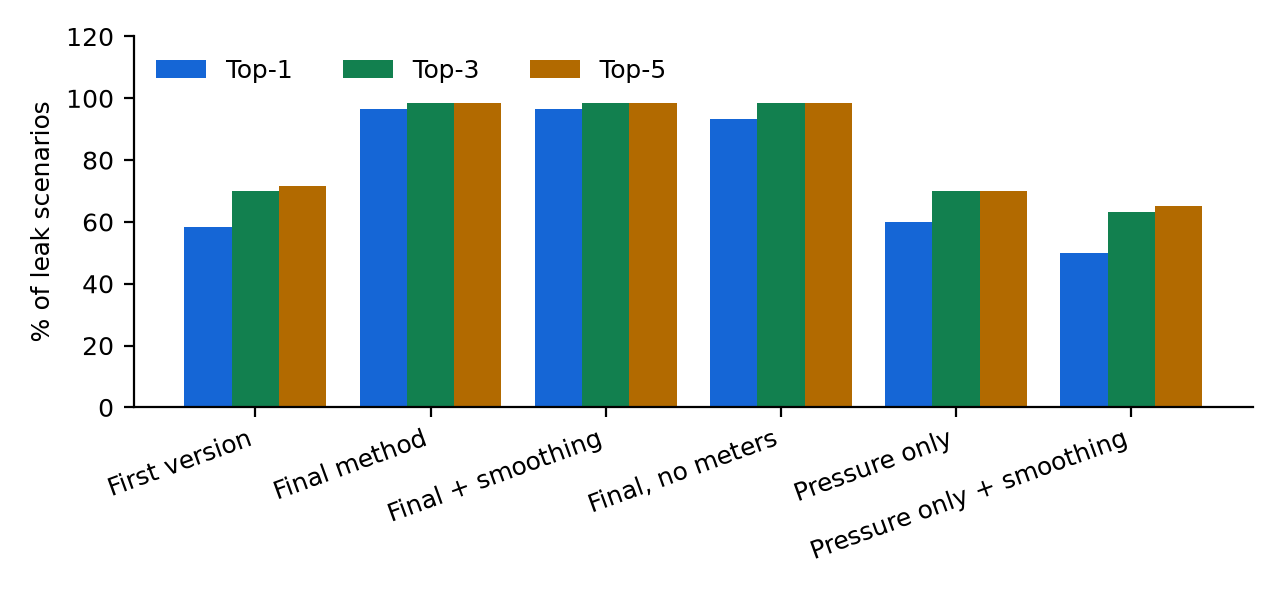
\includegraphics[width=0.85\linewidth]{figures/fig_localization.png}\caption{Localization accuracy of each method over all leak scenarios.}\end{figure}
Reading the table: using unaccounted flow lifts Top-1 from 58.3\% to 96.7\%. Without demand meters Top-1 is 93.3\%, because a demand change at another node can look like a small leak. Pressure alone gives only 60.0\%, because the drop spreads to neighbours. Smoothing scores over neighbouring nodes gave 96.7\%, no improvement, so the final method does not use it.

By scenario type, node type and network (final method, test leaks only; small groups):
\begin{center}\small\begin{tabular}{@{}lcccc@{}}\toprule
Group & Leaks & Top-1 & Top-5 & Mean hops \\\midrule
Leak hidden behind another event & 10 & 100.0\% & 100.0\% & 0.00 \\
Leak with sensor noise & 4 & 100.0\% & 100.0\% & 0.00 \\
Leak size sweep & 20 & 90.0\% & 95.0\% & 0.40 \\
Leak start time & 4 & 100.0\% & 100.0\% & 0.00 \\
Leak at every junction & 22 & 100.0\% & 100.0\% & 0.00 \\
\midrule
dead-end & 17 & 100.0\% & 100.0\% & 0.00 \\
hub & 1 & 100.0\% & 100.0\% & 0.00 \\
inline & 42 & 95.2\% & 97.6\% & 0.19 \\
net1 & 11 & 100.0\% & 100.0\% & 0.00 \\
net2 & 26 & 92.3\% & 96.2\% & 0.31 \\
net3 & 23 & 100.0\% & 100.0\% & 0.00 \\
\bottomrule\end{tabular}\end{center}
Why they differ:
\begin{itemize}[leftmargin=*,itemsep=2pt]
\item \emph{Size.} Large leaks are easy to notice but the biggest (0.01 m$^2$) drops pressure across the whole network and can wipe out the unaccounted-flow signal (in the NET2 example the exact node was ranked 14th), so the exact node is harder to pick. Tiny leaks sit close to the sensor noise, so some are reported as normal and the dashboard then shows no ranking.
\item \emph{Hidden behind another event.} A hydrant or pump outage at the same time adds pressure changes elsewhere; the unaccounted-flow signal is unaffected when demands are metered, so these stay accurate.
\item \emph{Topology.} Hubs and dead ends behave differently; a hub's neighbours share its pressure drop, which is why pressure-only localization struggles there.
\item \emph{Network.} Net1 is tiny (9 junctions), so a ``miss'' is never far from the truth.
\end{itemize}
\begin{figure}[H]\centering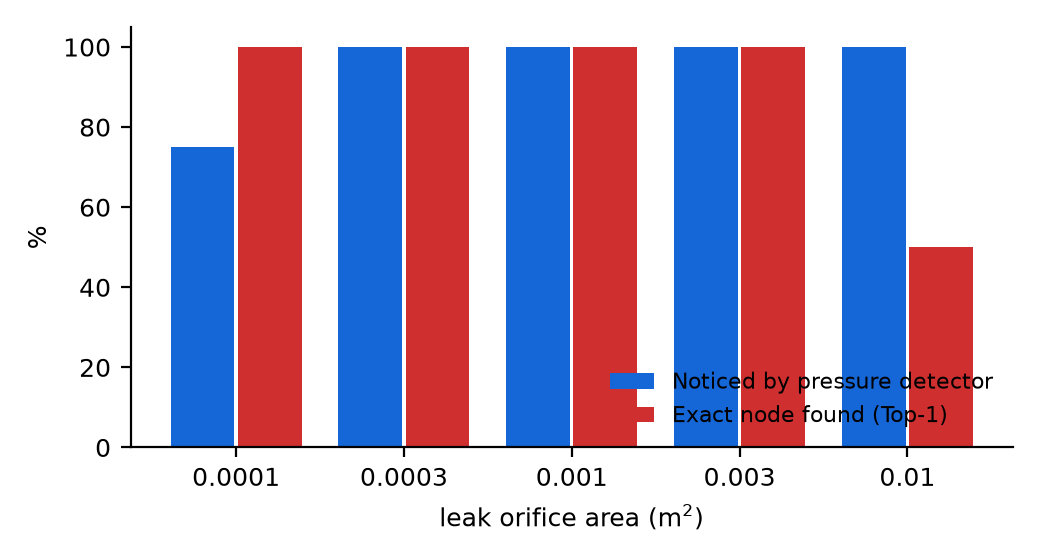
\includegraphics[width=0.62\linewidth]{figures/fig_size.png}\caption{Effect of leak size on detection and on finding the exact node.}\end{figure}

\section{How the other verdicts are reached}
\begin{itemize}[leftmargin=*,itemsep=3pt]
\item \term{Demand change}: pressure falls, but the unaccounted flow is near zero and the metered demand changed. \item \term{Pump or reservoir}: a pump's flow drops, or supply from the reservoirs changes, and most junctions lose pressure. \item \term{Tank change}: the tanks' net flow differs from normal. \item \term{Blocked pipe}: some junctions lose pressure while others gain it and many pipe flows change, with no unaccounted loss. \item \term{Pipe ageing}: a wide, smooth pressure loss with larger drops where flow is higher and no unaccounted loss.
\end{itemize}
\begin{figure}[H]\centering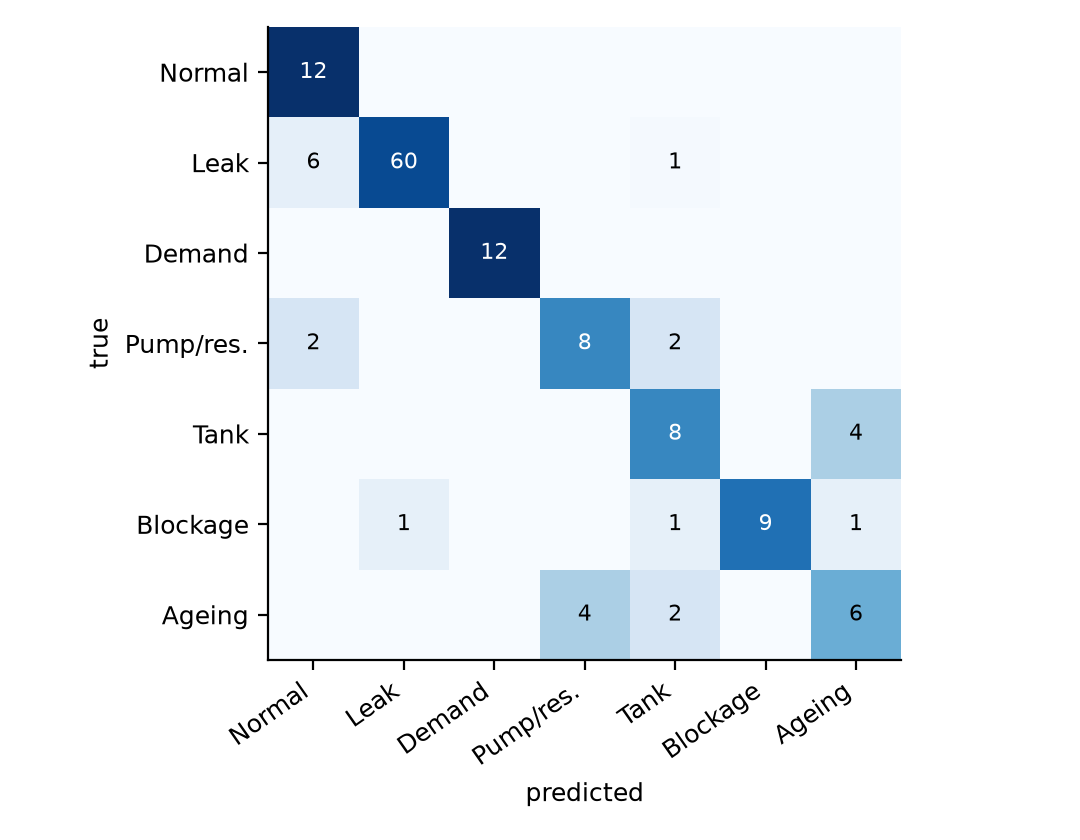
\includegraphics[width=0.62\linewidth]{figures/fig_confusion.png}\caption{Which cause the system names for each true cause (counts, held-out test scenarios).}\end{figure}
Leaks and demand changes are recognised very reliably. Pump, tank, blockage and ageing are sometimes confused with each other, because each makes the whole network lose pressure; and small events inside the noise are reported as normal.

\section{What the Performance tab shows}
It repeats these held-out test results in plain language, with the train-versus-test accuracy shown next to each other: leaks found at the exact node, leaks in the first five nodes, false alarms on normal days, right cause identified, the effect of leak size, the confusion between causes, results on a network the model has not seen (leave-one-network-out), and detailed per-group tables. The unseen-network results are weaker for fine-grained non-leak causes; this is the main work left for Semester 2.

\section{Limits to keep in mind}
\begin{itemize}[leftmargin=*,itemsep=2pt]
\item All data are simulated; real networks add noise and surprises.
\item The test set is small (139 scenarios, 60 scored leaks), so every percentage has a wide margin of error.
\item The leak-ranking settings and the 0.3 weight were chosen while looking at all scenarios, before the split was made; they were not re-tuned afterwards.
\item Separating a leak from a demand change relies on smart demand meters at the nodes.
\item Leaks that stay inside the sensor noise cannot be seen.
\item Net3 nodes 61 and 601 and hour 21 are ignored because their pressure swings wildly for a tiny change (pump switching).
\end{itemize}
\end{document}
